
If the three vertices are located at\begin{align}
     \vec{A},\vec{B},\vec{C}
\end{align} 
and the sides opposite these vertices have corresponding lengths \begin{align}
{a}, {b}\quad and\quad {c} 
\end{align} 
then:\\
 The coordinates of the centre of the Inscribed circle
 \begin{align}
 \vec{O}=\frac{1}{{a}+{b}+{c}}\myvec{{a}\vec{A}+{b} \vec{B}+{c}\vec{C}}
 \end{align} 
And the coordinates of the centre of the Escribed circle  opposite to the vertex $\vec{A}$
 \begin{align}
\vec{P}=\frac{1}{{b}+{c}-{a}}\myvec{ {b}\vec{B}+{c}\vec{C}-{a}\vec{A}}
 \end{align}
 
 The vertices $\vec{A}$ is the intersection of the sides $\vec{AB}$ and $\vec{CA}$.Thus $\vec{A}$ is obtained from
 \begin{align}
 \myvec{4\quad-3\\0\quad1}x=\myvec{12\\2}
 \end{align}
 The augmented matrix for the above equation is row reduced as follows
 \begin{align}
 \myvec{4\quad-3\quad 12\\0\quad1\quad2}\xleftrightarrow{R_1=R_1+3R_2}\myvec{4\quad0\quad 18\\0\quad1\quad2}\\\xleftrightarrow{R_1=\frac{1}{4}R_1}\myvec{1\quad0\quad\frac{9}{2}\\0\quad1\quad2}\\
 \Longrightarrow\vec{A}=\myvec{\frac{9}{2}\\2}
 \end{align}
 
  The vertices $\vec{B}$ is the intersection of the sides $\vec{AB}$ and $\vec{BC}$.Thus $\vec{B}$ is obtained from
 \begin{align}
 \myvec{4\quad-3\\3\quad4}x=\myvec{12\\24}
 \end{align}
 The augmented matrix for the above equation is row reduced as follows
 \begin{align}
 \myvec{4\quad-3\quad 12\\3\quad4\quad24}\xleftrightarrow{R_2=4R_2-3R_1}\myvec{4\quad-3\quad 12\\0\quad25\quad60}\\\xleftrightarrow{R_2=\frac{1}{25}R_2}\myvec{4\quad-3\quad 12\\0\quad1\quad\frac{12}{5}}\xleftrightarrow{R_1=R_1+3R_2}\myvec{4\quad0\quad\frac{96}{5}\\0\quad1\quad\frac{12}{5}}\\
 \xleftrightarrow{R_1=\frac{1}{4}R_1}\myvec{1\quad0\quad\frac{24}{5}\\0\quad1\quad\frac{12}{5}}\\
 \Longrightarrow\vec{B}=\myvec{\frac{24}{5}\\\frac{12}{5}}
 \end{align}
 The vertices $\vec{C}$ is the intersection of the sides $\vec{BC}$ and$\vec{CA}$.Thus $\vec{C}$ is obtained from
 \begin{align}
 \myvec{3\quad4\\0\quad 1}x=\myvec{24\\2}
 \end{align}
 The augmented matrix for the above equation is row reduced as follows
\begin{align}
 \myvec{3\quad4\quad 24\\0\quad1\quad2}\xleftrightarrow{R_1=R_1-4R_2}\myvec{3\quad0\quad 16\\0\quad1\quad2}\\\xleftrightarrow{R_1=\frac{1}{3}R_1}\myvec{1\quad0\quad\frac{16}{3}\\0\quad1\quad2}\\
 \Longrightarrow\vec{C}=\myvec{\frac{16}{3}\\2}
 \end{align}
 The length of the side $\vec{AB}$
 \begin{equation}
  {c}=\norm{(\vec{B}-\vec{A})}\\
    =\norm{\myvec{\frac{24}{5}\\\frac{12}{5}}-\myvec{\frac{9}{2}\\2}}\\
    =0.5
\end{equation}
 The length of the side $\vec{BC}$
 \begin{equation}
  {a}=\norm{(\vec{C}-\vec{B})}\\
    =\norm{\myvec{\frac{16}{3}\\2}-\myvec{\frac{24}{5}\\\frac{12}{5}}}\\
    =0.666
\end{equation}
  The length of the side $\vec{CA}$ 
  \begin{equation}
  {b}=\norm{(\vec{A}-\vec{C})}\\
    =\norm{\myvec{\frac{9}{2}\\2}-\myvec{\frac{16}{3}\\2}}\\
    =0.833
\end{equation}
 
Therefore the coordinates of the centre of the Inscribed circle
 \begin{align}
 \vec{O}=\frac{1}{.666+.833+0.5}\myvec{0.666\myvec{\frac{9}{2}\\2}+ 0.833\myvec{\frac{24}{5}\\\frac{12}{5}}+.5\myvec{\frac{16}{3}\\2}}\\
={\myvec{4.833\\2.166}}
 \end{align} 
And the coordinates of the centre of the Escribed circle  opposite to the vertex $\vec{A}$
 \begin{align}
\vec{P}=\frac{1}{.833+0.5-.666}\myvec{0.833\myvec{\frac{24}{5}\\\frac{12}{5}}+.5\myvec{\frac{16}{3}\\2}-0.666\myvec{\frac{9}{2}\\2}}\\
={\myvec{5.499\\2.499}}
 \end{align}

See Fig.     \ref{eq:solutions/2/4/8/myfig:1}

\begin{figure}[!]
 \begin{center}
  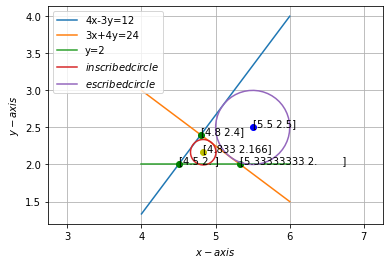
\includegraphics[width=\columnwidth]{solutions/2/4/8/assignment4_fig.png}
    \caption{This is the 2D diagram of the triangle , the inscribed circle and the escribed circle opposite to vertex $\vec{A}$}
    \label{eq:solutions/2/4/8/myfig:1}
    \end{center}
\end{figure}
